\documentclass[]{elsarticle} %review=doublespace preprint=single 5p=2 column
%%% Begin My package additions %%%%%%%%%%%%%%%%%%%
\usepackage[hyphens]{url}

  \journal{Science of Remote Sensing} % Sets Journal name


\usepackage{lineno} % add
\providecommand{\tightlist}{%
  \setlength{\itemsep}{0pt}\setlength{\parskip}{0pt}}

\usepackage{graphicx}
\usepackage{booktabs} % book-quality tables
%%%%%%%%%%%%%%%% end my additions to header

\usepackage[T1]{fontenc}
\usepackage{lmodern}
\usepackage{amssymb,amsmath}
\usepackage{ifxetex,ifluatex}
\usepackage{fixltx2e} % provides \textsubscript
% use upquote if available, for straight quotes in verbatim environments
\IfFileExists{upquote.sty}{\usepackage{upquote}}{}
\ifnum 0\ifxetex 1\fi\ifluatex 1\fi=0 % if pdftex
  \usepackage[utf8]{inputenc}
\else % if luatex or xelatex
  \usepackage{fontspec}
  \ifxetex
    \usepackage{xltxtra,xunicode}
  \fi
  \defaultfontfeatures{Mapping=tex-text,Scale=MatchLowercase}
  \newcommand{\euro}{€}
\fi
% use microtype if available
\IfFileExists{microtype.sty}{\usepackage{microtype}}{}
\bibliographystyle{elsarticle-harv}
\usepackage{graphicx}
% We will generate all images so they have a width \maxwidth. This means
% that they will get their normal width if they fit onto the page, but
% are scaled down if they would overflow the margins.
\makeatletter
\def\maxwidth{\ifdim\Gin@nat@width>\linewidth\linewidth
\else\Gin@nat@width\fi}
\makeatother
\let\Oldincludegraphics\includegraphics
\renewcommand{\includegraphics}[1]{\Oldincludegraphics[width=\maxwidth]{#1}}
\ifxetex
  \usepackage[setpagesize=false, % page size defined by xetex
              unicode=false, % unicode breaks when used with xetex
              xetex]{hyperref}
\else
  \usepackage[unicode=true]{hyperref}
\fi
\hypersetup{breaklinks=true,
            bookmarks=true,
            pdfauthor={},
            pdftitle={Sentinel-1 backscatter for forest analysis: can we push the limit?},
            colorlinks=false,
            urlcolor=blue,
            linkcolor=magenta,
            pdfborder={0 0 0}}
\urlstyle{same}  % don't use monospace font for urls

\setcounter{secnumdepth}{0}
% Pandoc toggle for numbering sections (defaults to be off)
\setcounter{secnumdepth}{0}


% Pandoc header



\begin{document}
\begin{frontmatter}

  \title{Sentinel-1 backscatter for forest analysis: can we push the limit?}
    \author[CIRGEO Interdepartmental Research Center of Research of Geomatics]{Francesco Pirotti\corref{1}}
   \ead{francesco.pirotti@unipd.it} 
    \author[TESAF Department]{Francesco Pirotti\corref{2}}
   \ead{francesco.pirotti@unipd.it} 
      \address[CIRGEO Interdepartmental Research Center of Research of Geomatics]{Agripolis, University of Padova, Legnaro 35020, Italy}
    \address[TESAF Department]{University of Padova, Legnaro 35020, Italy}
      \cortext[1]{Corresponding Author}
    \cortext[2]{Equal contribution}
  
  \begin{abstract}
  This is the abstract. It consists of two paragraphs.
  \end{abstract}
  
 \end{frontmatter}

\hypertarget{introduction}{%
\section{Introduction}\label{introduction}}

In this work the backscatter response of Sentinel-1 C-band signal over
forests is analysed to understand to what extent it can be used.
Numerous authors have investigated Sentinel-1 for forest analysis,
mostly in specific applications. This work wants to partially review
past results and provide novel information on how to use backscatter
information on forest cover.

Forests are a critical asset of our Earth balance. Forest cover and
composition change cyclically over long periods, more drastically after
natural or man-induced events such as fires, windthrow and straight tree
harvesting.

Cyclical changes in vegetation is a well-known fact. Most research
investigates fisiological changes connected to photosynthesis and
climate over seasons. Interestingly even physical position/orientation
of leaves and branches can reflect day/night (circadian leaf movements)
in birch trees (Puttonen et al.,
\protect\hyperlink{ref-Puttonen2016}{2016}).

The forest cover balance is important to monitor for well-known reasons
{[}manu citations here{]}. Optical remote sensing can provide a global
watch over land cover in general and forest cover in particular (Hansen
et al., \protect\hyperlink{ref-Hansen2013}{2013}; Margono et al.,
\protect\hyperlink{ref-Margono2014}{2014}).

The known limitation of optical remote sensing is noise from atmospheric
elements that cannot be corrected, mainly clouds and smoke. Active
remote sensing emits wavelengths that are not significantly influenced
by atmospheric conditions and can provide a very helpful complement to
optical remote sensing. Radar sensors have been widely used to study
vegetation cover, leveraging correlation between backscatter responses
and vegetative stage and vegetation type. Unfortunately several other
factors influence the return backscatter intensity, the main ones being
(i) incidence angle (ii) water content changing the (iii) di-electric
constant, (iv) snow/dust cover.

Below the points that are analysed:

\begin{itemize}
\tightlist
\item
  mitigating the effect of irregular terrain ie. mixed incidence angle
\item
  checking and removing any effect of seasonality
\item
  define how tree categories influence backscatter
\item
  detecting damaged forests, from

  \begin{itemize}
  \tightlist
  \item
    pathogens effecting the foliage
  \item
    windstorms
  \end{itemize}
\end{itemize}

In tropical forests Sentinel 1 and FIRMS has been used (Reiche et al.,
\protect\hyperlink{ref-Reiche2018}{2018})

\hypertarget{material-and-methods}{%
\section{Material and methods}\label{material-and-methods}}

The first step consisted the creation of a mask that isolates cells in
the study area that were covered more than 95\% with tree canopy and
that were subject to more than 90\% damage from VAIA storm. Furthermore
the cell must be part of a damaged site whose area was larger than
\(25000\ m^2\) The data consist in Sentinel 1 VV and VH backscatter
values only from these masked cells. ie. that have the following
characteristics:

\begin{itemize}
\item
  are completely (\textgreater{}95\%) covered by tree canopy - for this
  the forest cover map from 2000 (Hansen et al.,
  \protect\hyperlink{ref-Hansen2013}{2013}) was used by selecting only
  cells withe value 100 (100\% cover) and removing the ones that
  recorded loss between the period 2000-2019
\item
  are not covered by snow at time of recording - this was done by
  removing analysis of the closest Sentinel 2 image before the date of
  each Sentinel 1 image.
\item
  are damaged from VAIA's storm - for this the areas with forest loss
  defined in 2019 from (Hansen et al.,
  \protect\hyperlink{ref-Hansen2013}{2013}) that intersect the areas
  from (Forzieri et al., \protect\hyperlink{ref-Forzieri2020}{2020})
  with \textgreater{} 80\% damage.
\end{itemize}

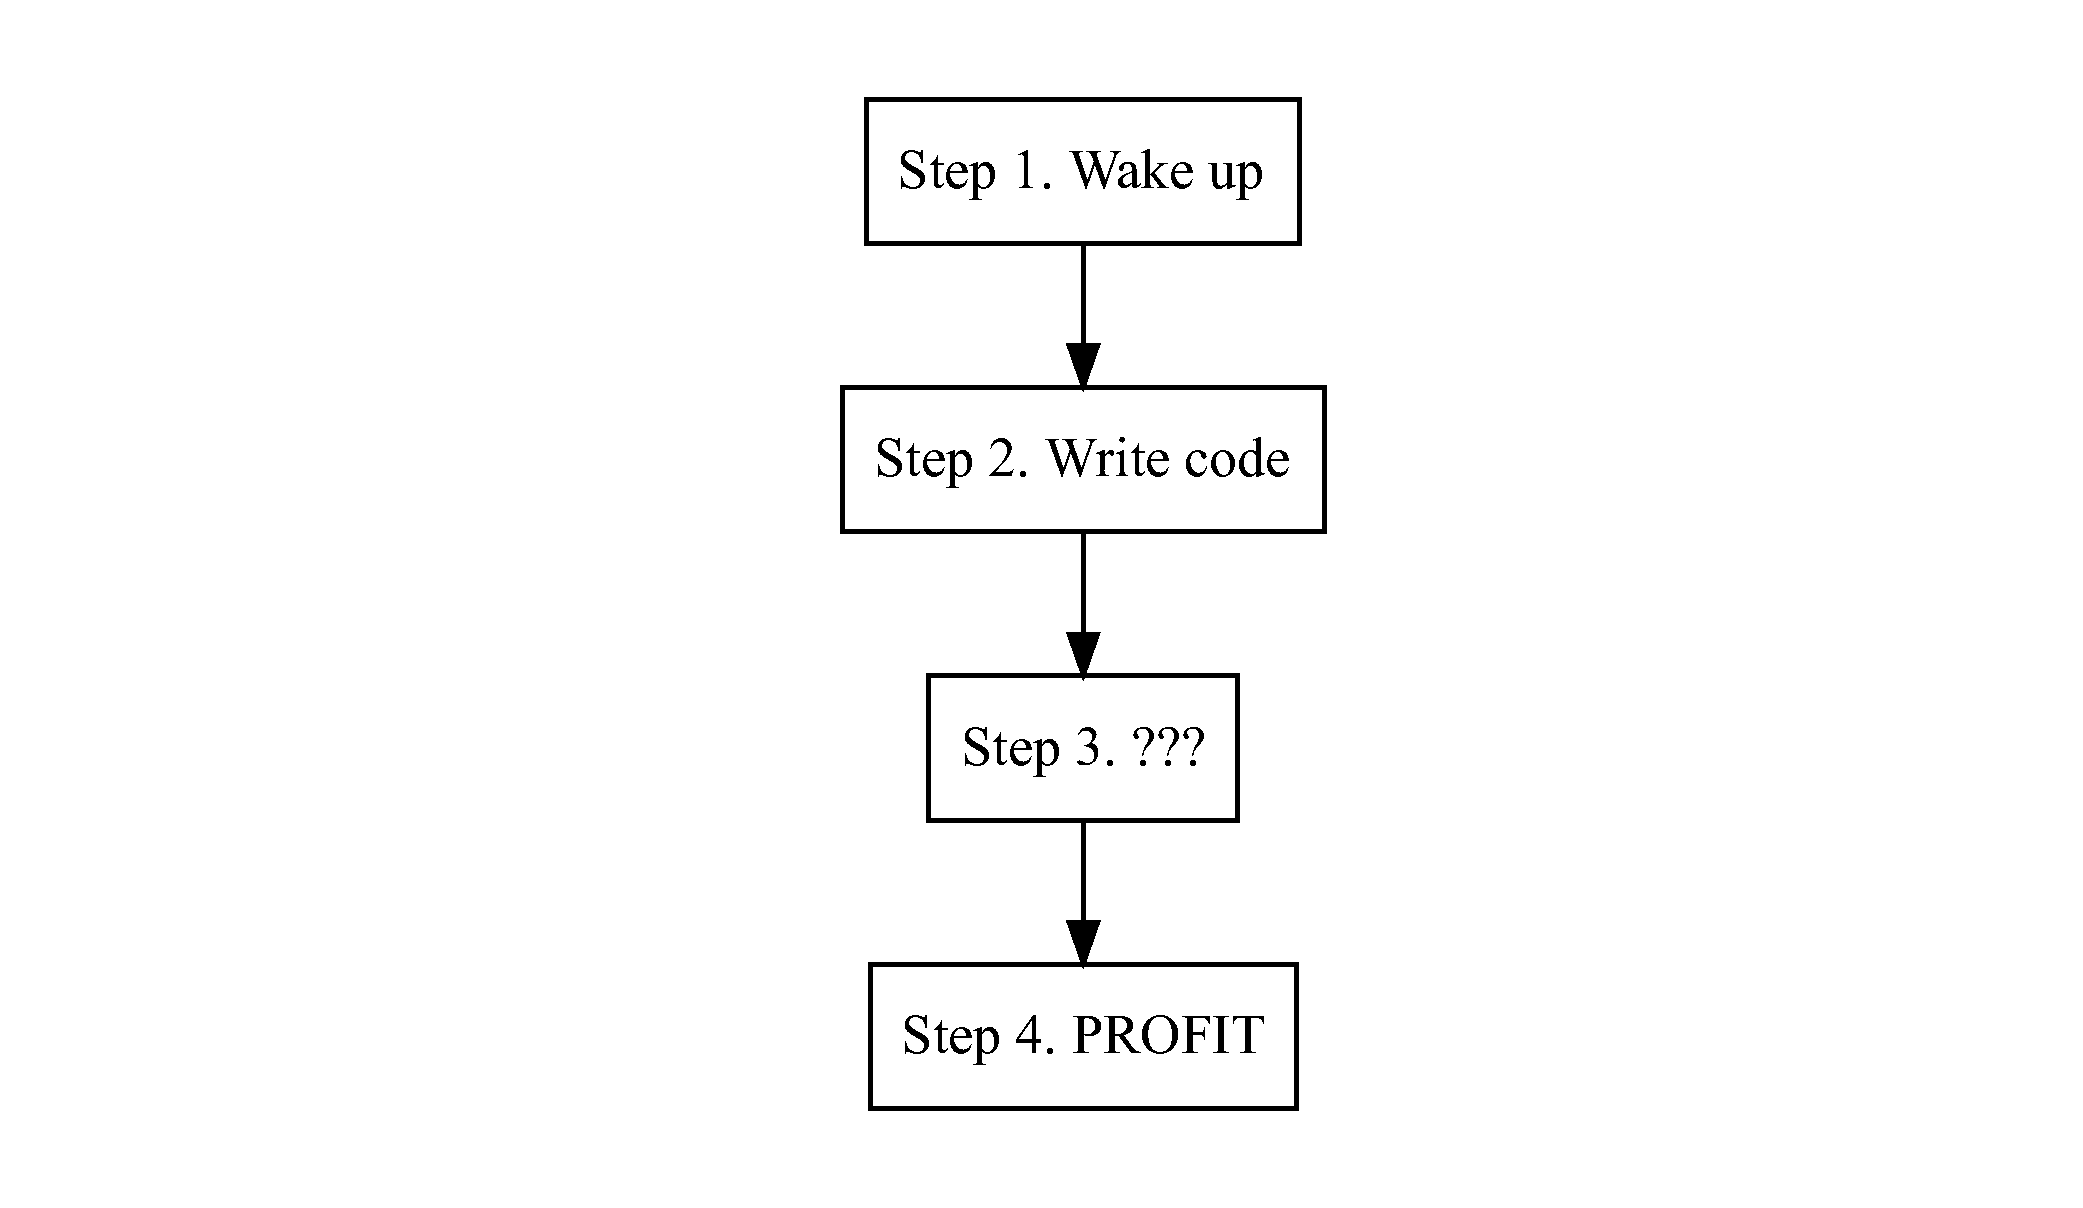
\includegraphics{paper2_files/figure-latex/unnamed-chunk-1-1.pdf}

\hypertarget{theorycalculation}{%
\section{Theory/calculation}\label{theorycalculation}}

\hypertarget{sentinel-1}{%
\subsection{Sentinel 1}\label{sentinel-1}}

Google Earth Engine (GEE) provides Sentinel 1 in preprocessed GRD
products with \(\sigma^0\) (sigma-naught) of VV and VH polarizations,
after processing for removing thermal noise, calibrating radiometry and
converting \(\beta^0\) beta-naught to sigma-naught using a digital
elevation model (DEM). The DEM at the latitudes of the analysed study
areas used is from the Shuttle Radar Topography Mission (SRTM) that took
place in february 2000 ({\textbf{???}}). Sigma-naught is provided in dB
by transformation the backscatter value \(Y=10*log_{10}(X)\) . Small
(\protect\hyperlink{ref-Small2011}{2011}). The GEE product was further
transformed to provide gamma-naught (\(\gamma^0\)) values, thus
correcting for the local incidence angle with the SRTM product. This
removed the bias between ascending and descenging orbits that was
evident from plotting the data.

Incidence angle was further corrected using a frequency-histogram based
mehod as described in (Mladenova et al.,
\protect\hyperlink{ref-Mladenova2013}{2013}). This method is not
site-specific or sensor-dependant. Is has also proven to be effective
not only for small incidence angles, which is the case here as the area
is over mountainous region.

\hypertarget{palsar-2}{%
\subsection{PALSAR-2}\label{palsar-2}}

Polarization data are stored in GEE as 16-bit digital numbers (DN). As
per indication in the GEE website, the DN values can be converted to
gamma naught (\(\gamma^0\)) values in decibel unit (dB) using the
following equation:

\[
\begin{aligned}
 \gamma^0 = 10*log_{10}(DN) - 83.0  
\end{aligned}
\]

where \(83.0 \  dB\) offset and \(\gamma^0\) is in dB.

values, thus correcting for the local incidence angle with the SRTM
product.

\hypertarget{results}{%
\section{Results}\label{results}}

\hypertarget{discussion}{%
\section{Discussion}\label{discussion}}

\hypertarget{conclusions}{%
\section{Conclusions}\label{conclusions}}

\hypertarget{acknowledgements}{%
\section{Acknowledgements}\label{acknowledgements}}

This effort is also part of the
\href{https://www.tesaf.unipd.it/ricerca/progetti-dip-tesaf}{VAIA FRONT
project - FRom lessong learned to future Options} .

\hypertarget{bibliography-styles}{%
\section{Bibliography styles}\label{bibliography-styles}}

There are various bibliography styles available. You can select the
style of your choice in the preamble of this document. These styles are
Elsevier styles based on standard styles like Harvard and Vancouver.
Please use BibTeX~to generate your bibliography and include DOIs
whenever available.

\hypertarget{references}{%
\section*{References}\label{references}}
\addcontentsline{toc}{section}{References}

\hypertarget{refs}{}
\leavevmode\hypertarget{ref-Forzieri2020}{}%
Forzieri, G., Pecchi, M., Girardello, M., Mauri, A., Klaus, M., Nikolov,
C., Rüetschi, M., Gardiner, B., Tomaštík, J., Small, D., Nistor, C.,
Jonikavicius, D., Spinoni, J., Feyen, L., Giannetti, F., Comino, R.,
Wolynski, A., Pirotti, F., Maistrelli, F., Savulescu, I.,
Wurpillot-Lucas, S., Karlsson, S., Zieba-Kulawik, K.,
Strejczek-Jazwinska, P., Mokroš, M., Franz, S., Krejci, L., Haidu, I.,
Nilsson, M., Wezyk, P., Catani, F., Chen, Y.-Y., Luyssaert, S., Chirici,
G., Cescatti, A., Beck, P.S.A., 2020. A spatially explicit database of
wind disturbances in European forests over the period 2000 - 2018. Earth
System Science Data 12, 257--276.
doi:\href{https://doi.org/10.5194/essd-12-257-2020}{10.5194/essd-12-257-2020}

\leavevmode\hypertarget{ref-Hansen2013}{}%
Hansen, M.C., Potapov, P.V., Moore, R., Hancher, M., Turubanova, S.A.,
Tyukavina, A., Thau, D., Stehman, S.V., Goetz, S.J., Loveland, T.R.,
Kommareddy, A., Egorov, A., Chini, L., Justice, C.O., Townshend, J.R.G.,
2013. High-Resolution Global Maps of 21st-Century Forest Cover Change.
Science 342, 850--853.
doi:\href{https://doi.org/10.1126/science.1244693}{10.1126/science.1244693}

\leavevmode\hypertarget{ref-Margono2014}{}%
Margono, B.A., Potapov, P.V., Turubanova, S., Stolle, F., Hansen, M.C.,
2014. Primary forest cover loss in Indonesia over 2000--2012. Nature
Climate Change 4, 730--735.
doi:\href{https://doi.org/10.1038/nclimate2277}{10.1038/nclimate2277}

\leavevmode\hypertarget{ref-Mladenova2013}{}%
Mladenova, I.E., Jackson, T.J., Bindlish, R., Hensley, S., 2013.
Incidence Angle Normalization of Radar Backscatter Data. IEEE
Transactions on Geoscience and Remote Sensing 51, 1791--1804.
doi:\href{https://doi.org/10.1109/TGRS.2012.2205264}{10.1109/TGRS.2012.2205264}

\leavevmode\hypertarget{ref-Puttonen2016}{}%
Puttonen, E., Briese, C., Mandlburger, G., Wieser, M., Pfennigbauer, M.,
Zlinszky, A., Pfeifer, N., 2016. Quantification of Overnight Movement of
Birch (Betula pendula) Branches and Foliage with Short Interval
Terrestrial Laser Scanning. Frontiers in Plant Science 7.
doi:\href{https://doi.org/10.3389/fpls.2016.00222}{10.3389/fpls.2016.00222}

\leavevmode\hypertarget{ref-Reiche2018}{}%
Reiche, J., Verhoeven, R., Verbesselt, J., Hamunyela, E., Wielaard, N.,
Herold, M., 2018. Characterizing Tropical Forest Cover Loss Using Dense
Sentinel-1 Data and Active Fire Alerts. Remote Sensing 10, 777.
doi:\href{https://doi.org/10.3390/rs10050777}{10.3390/rs10050777}

\leavevmode\hypertarget{ref-Small2011}{}%
Small, D., 2011. Flattening gamma: Radiometric terrain correction for
SAR imagery. IEEE Transactions on Geoscience and Remote Sensing.
doi:\href{https://doi.org/10.1109/TGRS.2011.2120616}{10.1109/TGRS.2011.2120616}


\end{document}


